\FloatBarrier

\begin{figure}[h!]
	\centering
	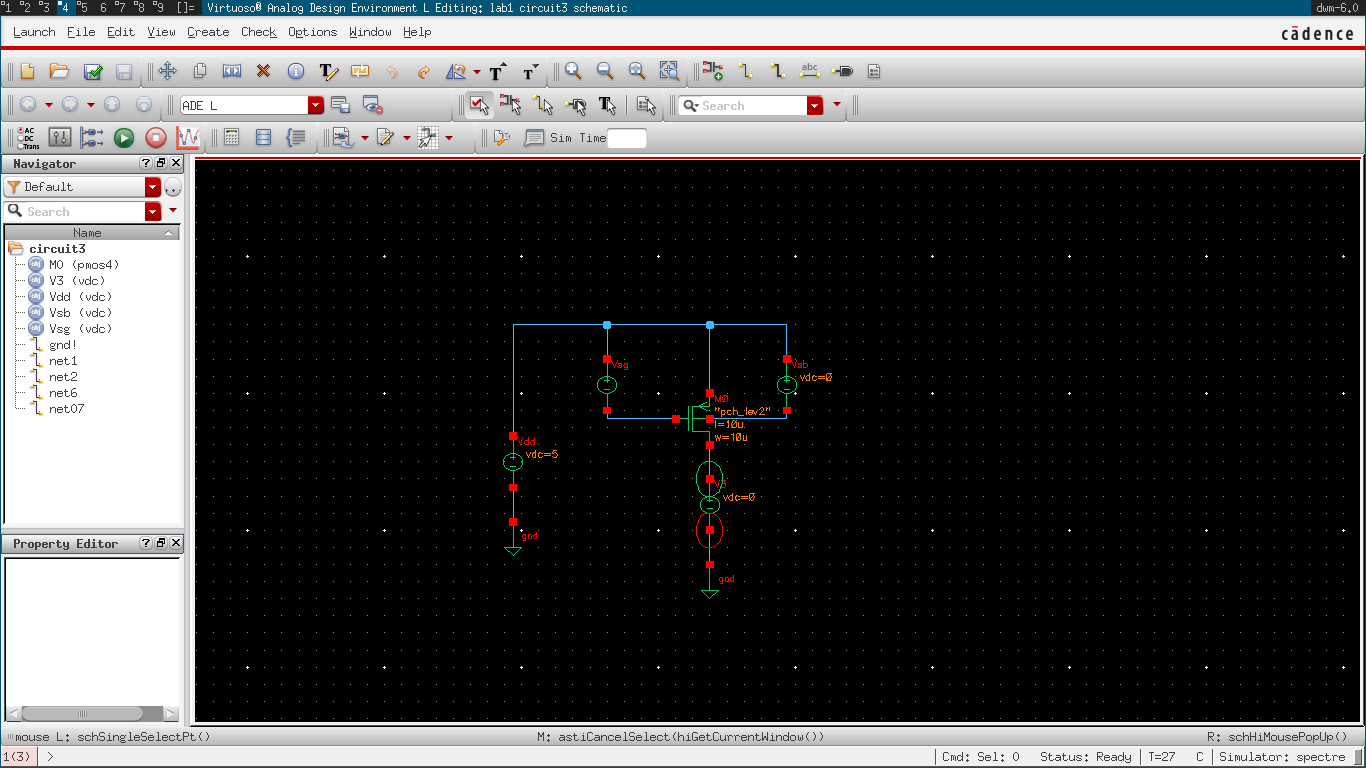
\includegraphics[scale=0.30]{../images/circuit3.PNG}
	\caption{Circuit for Simulation 3}
	\label{fig:circuit3}
\end{figure}

\FloatBarrier

Simulation 3 is similar to Simulation 1 except that a PMOS is used instead of an NMOS.

\FloatBarrier

\begin{figure}[h!]
	\centering
	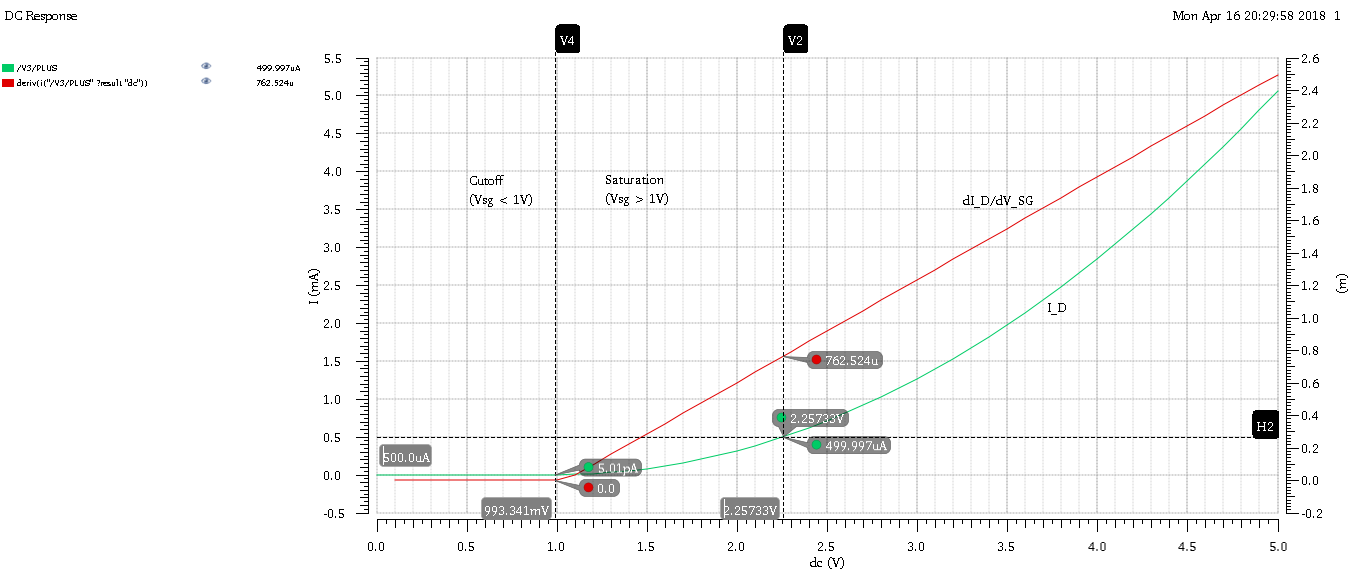
\includegraphics[scale=0.30]{../images/500ua_point_pmos.PNG}
	\caption{$I_{D}$ and $\frac{\partial I_{D}}{\partial V_{SG}}$ versus $V_{SG}$ for PMOS}
	\label{fig:id_vs_vgs_pmos}
\end{figure}

\FloatBarrier

Again, the transistor is in saturation when it exits cutoff because $V_{SD} = 5$\si{\volt} and $V_{SG} < 5$\si{\volt}, meaning $V_{SG} - |V_{t}| < V_{SD}$\si{\volt}.
For the PMOS, the definition $g_{m} = \frac{\partial I_{D}}{\partial V_{SG}}$ shall be used.

\FloatBarrier

\begin{table}[h!]
	\centering
	\caption{Simulation 3 Results}
	\label{tab:sim3_results}
	\csvautotabular{../tables/sim3_results}
\end{table}

\FloatBarrier
